\documentclass[border=3mm]{standalone}
\usepackage{tikz}
\usetikzlibrary{arrows, shapes.gates.logic.US, shapes.gates.logic.IEC, calc}

\tikzset{
    my-nand3-gate/.style={
        nand gate US, draw, rotate=0, logic gate inputs=nnn
    },
    my-branch/.style={
        fill, shape=circle, minimum size=3pt, inner sep=0pt
    },
}

\begin{document}

\resizebox{20cm}{!}{

    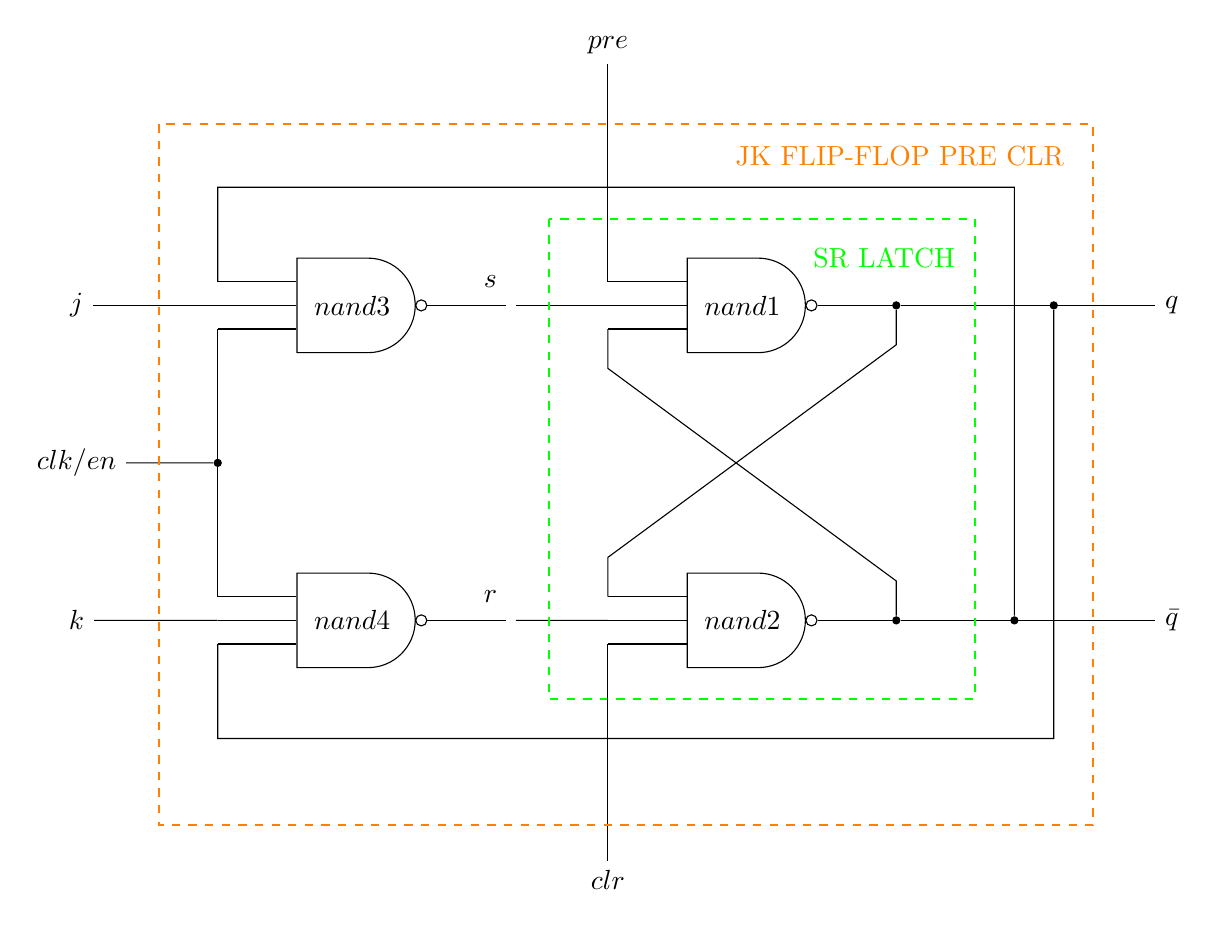
\begin{tikzpicture}[label distance=2mm]

        % JK FLIP-FLOP WITH PRESET AND CLEAR ----------------------------------------------------------

        % INPUTS - JK FLIP-FLOP WITH PRESET AND CLEAR
        \node[] (J)   at (0, 0)            {\normalsize $j$};
        \node[] (CLK) at ($(J) + (0, -2)$) {\normalsize $clk/en$};
        \node[] (K)   at ($(J) + (0, -4)$) {\normalsize $k$};

        % NAND3, WIRES AND CONNECTOR POINTS
        \node[my-nand3-gate](NAND3)    at ($(J) + (3.5, 0)$)            {\normalsize $nand3$};
        \coordinate[]       (NAND3IN1) at ($(NAND3.input 1) + (-1, 0)$) {};
        \coordinate[]       (NAND3IN2) at ($(NAND3.input 2) + (-1, 0)$) {};
        \coordinate[]       (NAND3IN3) at ($(NAND3.input 3) + (-1, 0)$) {};
        \coordinate[]       (NAND3OUT) at ($(NAND3.output)  + (1, 0)$)  {};
        \draw (NAND3.input 1) -- (NAND3IN1);
        \draw (NAND3.input 2) -- (NAND3IN2);
        \draw (NAND3.input 3) -- (NAND3IN3);
        \draw (NAND3.output)  -- (NAND3OUT);
        
        % NAND4, WIRES AND CONNECTOR POINTS
        \node[my-nand3-gate](NAND4)    at ($(K) + (3.5, 0)$)            {\normalsize $nand4$};
        \coordinate[]       (NAND4IN1) at ($(NAND4.input 1) + (-1, 0)$) {};
        \coordinate[]       (NAND4IN2) at ($(NAND4.input 2) + (-1, 0)$) {};
        \coordinate[]       (NAND4IN3) at ($(NAND4.input 3) + (-1, 0)$) {};
        \coordinate[]       (NAND4OUT) at ($(NAND4.output)  + (1, 0)$)  {};
        \draw (NAND4.input 1) -- (NAND4IN1);
        \draw (NAND4.input 2) -- (NAND4IN2);
        \draw (NAND4.input 3) -- (NAND4IN3);
        \draw (NAND4.output)  -- (NAND4OUT);

        % INPUT CONNECTIONS
        \draw (J) -- (NAND3IN2);
        \draw (K) -- (NAND4IN2);

        % INTERNAL WIRES - CLOCK
        \draw (NAND3IN3) -- (NAND4IN1) node[my-branch, pos=1/2] (CLKBRANCH) {};
        \draw (CLK) -- (CLKBRANCH);

        % SR LATCH ------------------------------------------------------------------------------------
        % POSITION AND ADJUST SPACING AND ADDED INPUT 3

        % INPUTS - SR LATCH
        \node[] (S) at ($(NAND3OUT) + (0, 0)$) {}; % *****POSITION*****
        \node[] (R) at ($(NAND4OUT) + (0, 0)$) {}; % *****POSITION*****

        % NAND1, WIRES AND CONNECTOR POINTS *****ADJUSTED SPACING AND ADDED INPUT 3*****
        \node[my-nand3-gate] (NAND1)   at ($(S) + (3, 0)$)              {\normalsize $nand1$};
        \coordinate[]       (NAND1IN1) at ($(NAND1.input 1) + (-1, 0)$) {};
        \coordinate[]       (NAND1IN2) at ($(NAND1.input 2) + (-1, 0)$) {};
        \coordinate[]       (NAND1IN3) at ($(NAND1.input 3) + (-1, 0)$) {};
        \node[my-branch]    (NAND1OUT) at ($(NAND1.output)  + (1, 0)$)  {};
        \draw (NAND1.input 1) -- (NAND1IN1);
        \draw (NAND1.input 2) -- (NAND1IN2);
        \draw (NAND1.input 3) -- (NAND1IN3);
        \draw (NAND1.output)  -- (NAND1OUT);
        
        % NAND2, WIRES AND CONNECTOR POINTS *****ADJUSTED SPACING AND ADDED INPUT 3*****
        \node[my-nand3-gate] (NAND2)   at ($(R) + (3, 0)$)              {\normalsize $nand2$};
        \coordinate[]       (NAND2IN1) at ($(NAND2.input 1) + (-1, 0)$) {};
        \coordinate[]       (NAND2IN2) at ($(NAND2.input 2) + (-1, 0)$) {};
        \coordinate[]       (NAND2IN3) at ($(NAND2.input 3) + (-1, 0)$) {};
        \node[my-branch]    (NAND2OUT) at ($(NAND2.output)  + (1, 0)$)  {};
        \draw (NAND2.input 1) -- (NAND2IN1);
        \draw (NAND2.input 2) -- (NAND2IN2);
        \draw (NAND2.input 3) -- (NAND2IN3);
        \draw (NAND2.output)  -- (NAND2OUT);

        % OUTPUTS - SR LATCH *****POSITION*****
        \node[] (Q)    at ($(NAND1OUT) + (3.5, 0)$) {\normalsize $q$};
        \node[] (QBAR) at ($(NAND2OUT) + (3.5, 0)$) {\normalsize $\bar{q}$};
                
        % INPUT WIRE CONNECTIONS
        \draw (S) -- (NAND1IN2);
        \draw (R) -- (NAND2IN2);
        
        % OUTPUT WIRE CONNECTIONS
        \draw (NAND1OUT) -- (Q);
        \draw (NAND2OUT) -- (QBAR);

        % INTERNAL WIRE CONNECTIONS
        \draw (NAND1OUT) -- ++(0,-0.5) -- ($(NAND2IN1) +(0,0.5)$)  -- (NAND2IN1);
        \draw (NAND2OUT) -- ++(0,0.5)  -- ($(NAND1IN3) +(0,-0.5)$) -- (NAND1IN3);

        % DRAW DOTTED LINE BOX AROUND SR LATCH
        \draw[thick, dashed, green] ($(NAND1IN1) + (-.75, .8)$) rectangle ($(NAND2OUT) + (1, -1)$);
        \node[green] at ($(NAND1) + (1.8, .6)$) {\normalsize SR LATCH};

        % JK FLIP-FLOP WITH PRESET AND CLEAR (CONTINUED) ----------------------------------------------

        % INPUTS (MORE INPUTS UP ABOVE)
        \node[] (PRE) at ($(NAND1IN1) + (0, 3)$)  {\normalsize $pre$};
        \node[] (CLR) at ($(NAND2IN3) + (0, -3)$) {\normalsize $clr$};

        % INPUT CONNECTIONS
        \draw (PRE) -- (NAND1IN1);
        \draw (CLR) -- (NAND2IN3);
        
        % INTERNAL WIRES
        \draw (NAND3OUT) -- (S);
        \node at ($(S) + (-.2, .3)$) {\normalsize $s$};
        \draw (NAND4OUT) -- (R);
        \node at ($(R) + (-.2, .3)$) {\normalsize $r$};

        % ADD ANOTHER NODE FOR OUTPUT FEEDBACK
        \node[my-branch] (NAND1OUTFEEDBACK) at ($(NAND1.output)  + (3, 0)$)  {};
        \node[my-branch] (NAND2OUTFEEDBACK) at ($(NAND2.output)  + (2.5, 0)$)  {};

        % INTERNAL WIRES - Q and QBAR FEEDBACK
        \draw (NAND1OUTFEEDBACK) -- ($(NAND2OUTFEEDBACK) + (.5,-1.5)$) -- ($(NAND4IN3) + (0,-1.2)$)  -- (NAND4IN3);
        \draw (NAND2OUTFEEDBACK) -- ($(NAND1OUTFEEDBACK) + (-.5,1.5)$) -- ($(NAND3IN1) + (0,1.2)$)   -- (NAND3IN1);

        % DRAW DOTTED LINE BOX AROUND JK FLIP-FLOP WITH PRESET AND CLEAR
        \draw[thick, dashed, orange] ($(NAND3IN1) + (-.75, 2)$) rectangle ($(NAND2OUT) + (2.5, -2.6)$);
        \node[orange] at ($(NAND1) + (2, 1.9)$) {\normalsize JK FLIP-FLOP PRE CLR};

    \end{tikzpicture}
}

\end{document} 
